\documentclass{beamer}
\usetheme{metropolis}
\usepackage{graphicx}
\usepackage{subfig}
\usepackage{tcolorbox}
\title{Algebra-Based Physics-2: Electricity, Magnetism, and Modern Physics (PHYS135B-01): Unit 3 Worksheet}
\author{Jordan Hanson}
\institute{Whittier College Department of Physics and Astronomy}

\begin{document}

\begin{frame}{Amp\`{e}re's Law}
\begin{figure}
\centering
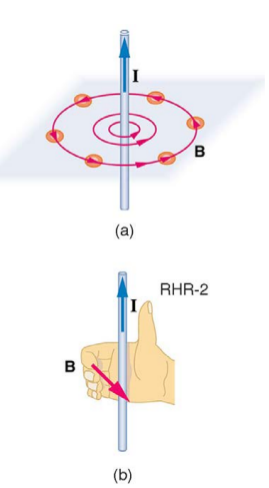
\includegraphics[width=0.15\textwidth]{figures/amplawrhr.png}
\caption{\label{fig:amplaw} \textit{Ampere's Law} gives several important results for B-fields generated by currents.}
\end{figure}
The uniform B-field of a wire of current I at a distance R is
\begin{equation}
\vec{B} = \frac{\mu_0 I}{2\pi R} \hat{\phi}
\end{equation}
\end{frame}

\begin{frame}{Amp\`{e}re's Law}
\begin{figure}
\centering
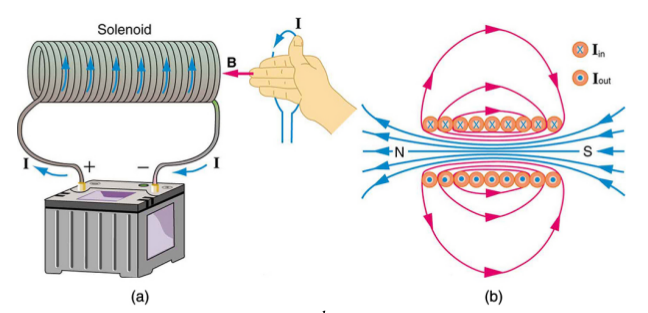
\includegraphics[width=0.75\textwidth]{figures/solenoid.png}
\caption{\label{fig:solenoid} A \textit{solenoid} creates a uniform B-field via \textit{Ampere's Law}.}
\end{figure}
The uniform B-field is proportional to the coils per unit length, and the current.
\begin{equation}
\vec{B} = \mu_0 \frac{N}{L} I \hat{x} = \mu_0 n I \hat{x}
\end{equation}
\end{frame}

\begin{frame}{Amp\`{e}re's Law}
\begin{enumerate}
\item How strong is the B-field strength inside a solenoid with 10,000 turns per meter that carries 20.0 A?
\item What is the B-field strength a distance of 1 m from a wire carrying a current of 1.0 A?
\item What is the field inside a 2.00-m-long solenoid that has 2000 loops and carries a 1600-A current?
\item Nonnuclear submarines use batteries for power when
submerged. (a) Find the magnetic field 50.0 cm from a
straight wire carrying 1200 A from the batteries to the drive
mechanism of a submarine. (b) What is the field if the wires to
and from the drive mechanism are side by side? (\textbf{Draw a diagram to help explain}). (c) Discuss
the effects this could have for a compass on the submarine
that is not shielded.
\end{enumerate}
\end{frame}

\end{document}
